\section{Performance Evaluation}\label{sec:evaluation}

We evaluate the computational overhead introduced by DSphinx and its scalability with respect to the two protocol parameters that dominate its computational cost: the path length $m$ and the reconstruction threshold $d$.

We implemented DSphinx in Python and Rust.\footnote{\artifact \newline The Rust version was developed in the context of a master's thesis as an independent implementation for cross-validation of Python implementation and results.}
The evaluation presented in this section uses the Python prototype, benchmarked on a laptop equipped with a 13th Gen Intel Core i7-13700HX CPU (3.70 GHz) and 32 GB of RAM.
The benchmark considers a network of 100 nodes, 50 STTPs, and 40 clients, where each client constructs a single DSphinx packet using the decentralized route-sampling protocol. 
We vary the path length $m \in \{3,4,5,6,7\}$ and the reconstruction threshold $d \in \{3,5,10,20\}$, resulting in 20 benchmark configurations. 
Network latency and communication overhead are intentionally excluded so that the measurements isolate the computational cost of the protocol.

\begin{figure}[t]
    \centering
    \begin{subfigure}{0.49\linewidth}
        \centering
        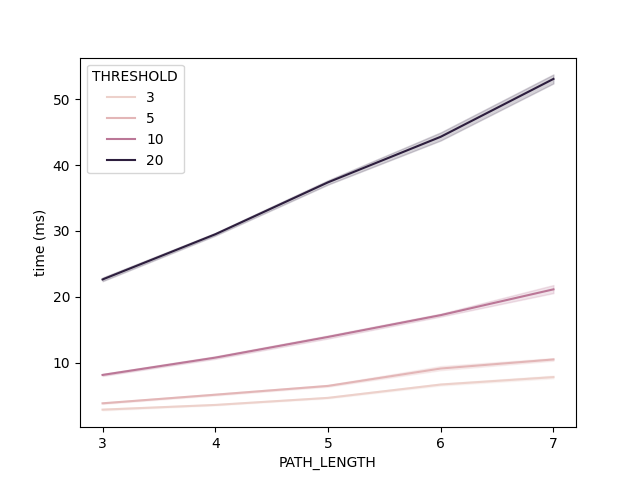
\includegraphics[width=\linewidth]{Images/path_length.png}
    \end{subfigure}
    \hfill
    \begin{subfigure}{0.49\linewidth}
        \centering
        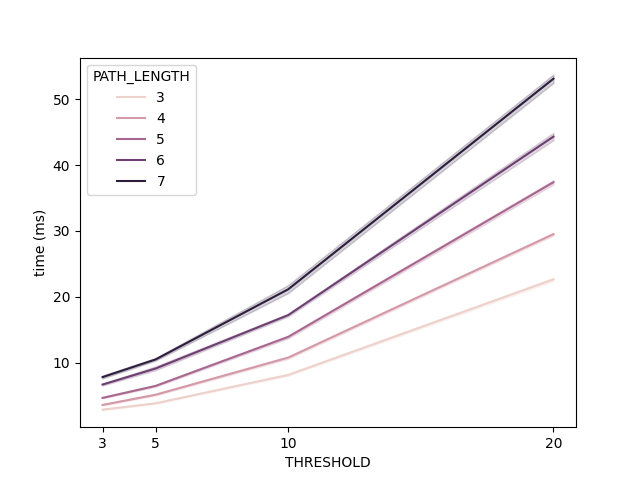
\includegraphics[width=\linewidth]{Images/threshold.png}
    \end{subfigure}
    \caption{Client-side execution time (ms) of DSphinx, including packet construction and decentralized route sampling, under varying path length ($m$) and reconstruction threshold ($d$).}
    \label{fig:scalability}
\end{figure}

Figure~\ref{fig:scalability} reports the total client-side runtime required for packet construction and decentralized route sampling. 
Depending on the parameter configuration, the runtime ranges from approximately 3 ms to 50 ms, compared to 0.5-2 ms for the original Sphinx.
The measured runtimes are consistent with the theoretical complexity of the protocol. 
In particular, the dominant cost arises from decentralized route sampling, whose threshold reconstruction requires $\mathcal{O}(d \log d)$ operations for each of the $m$ routing hops, yielding an overall client-side complexity of $\mathcal{O}(md \log d)$. 
This trend is clearly reflected in Figure~\ref{fig:scalability}, where increasing either the path length or the reconstruction threshold results in an approximately linear increase in execution time.

Figure~\ref{fig:runtime} summarizes the execution times of the main protocol phases and illustrates their dependence to path length $m$ and reconstruction threshold $d$.
On the client side, execution is dominated by decentralized route sampling, which accounts for approximately 86\% (approximately 2-50 ms) of the total runtime, whereas DSphinx packet construction contributes only the remaining 14\% (approximately 0.5-4.5 ms). 
On the network side, packet processing remains lightweight, requiring only 0.5-0.8 ms per packet, compared with approximately 0.15 ms for Sphinx. 
Although the node setup phase is the most computationally expensive operation (approximately 15-100 ms), it is performed only once during initialization.
Similarly, STTPs introduce only negligible computational overhead. 
Processing a route-sampling request requires approximately 0.3-0.7 ms, while the one-time setup phase completes in approximately 0.3 ms.

\begin{figure}[t]
    \centering
    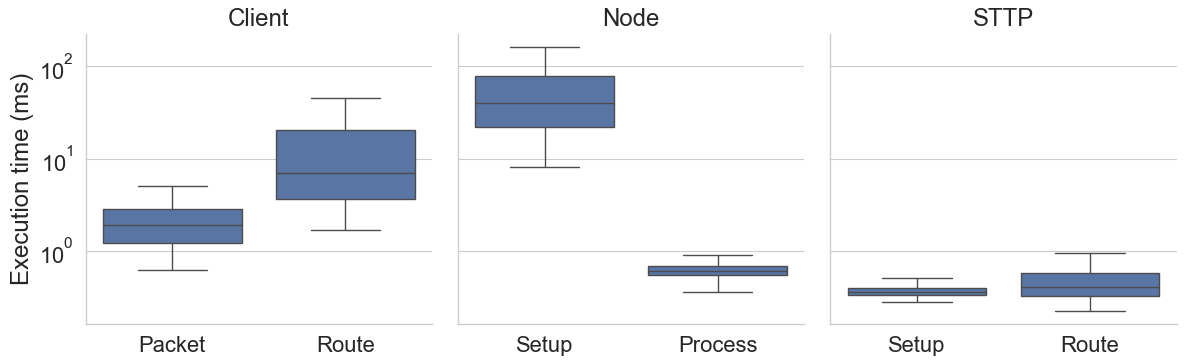
\includegraphics[width=\linewidth]{Images/boxplot.png}
    \caption{Execution times (ms) for DSphinx client, node, and STTP operations under varying path length $m$ and reconstruction threshold $d$.}
    \label{fig:runtime}
\end{figure}

Overall, the evaluation highlights the trade-off introduced by DSphinx. 
Although decentralized route sampling increases the client-side computational cost compared with Sphinx, the overhead remains modest in the context of deployed anonymous communication systems. 
Recent measurements of the Nym mixnet report end-to-end latencies of approximately 500-800 ms, largely dominated by mixing delays (around 50 ms per hop) and network propagation rather than cryptographic processing \cite{diaz2024reliability}. 
In comparison, the additional overhead introduced by DSphinx remains below 50 ms, making it unlikely to dominate end-to-end communication latency in practice.